% Graphic for TeX using PGF
% Title: C:\Users\josea\GitHub\IAL\diagramas_aplicacoes\exercicio_21-circuito-poole.dia
% Creator: Dia v0.97.2
% CreationDate: Mon Apr 17 21:04:35 2023
% For: josea
% \usepackage{tikz}
% The following commands are not supported in PSTricks at present
% We define them conditionally, so when they are implemented,
% this pgf file will use them.
\ifx\du\undefined
  \newlength{\du}
\fi
\setlength{\du}{15\unitlength}
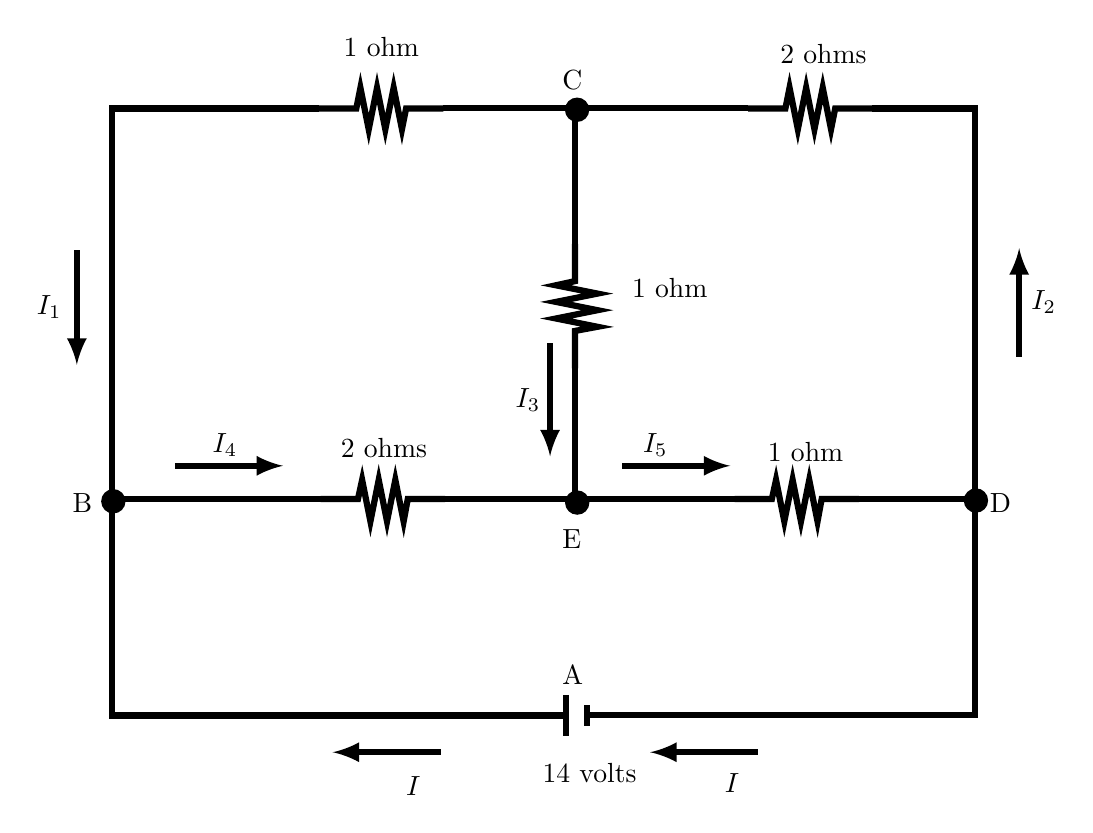
\begin{tikzpicture}
\pgftransformxscale{1.000000}
\pgftransformyscale{-1.000000}
\definecolor{dialinecolor}{rgb}{0.000000, 0.000000, 0.000000}
\pgfsetstrokecolor{dialinecolor}
\definecolor{dialinecolor}{rgb}{1.000000, 1.000000, 1.000000}
\pgfsetfillcolor{dialinecolor}
\pgfsetlinewidth{0.150000\du}
\pgfsetdash{}{0pt}
\pgfsetdash{}{0pt}
\pgfsetbuttcap
\pgfsetmiterjoin
\pgfsetlinewidth{0.150000\du}
\pgfsetbuttcap
\pgfsetmiterjoin
\pgfsetdash{}{0pt}
\definecolor{dialinecolor}{rgb}{0.000000, 0.000000, 0.000000}
\pgfsetstrokecolor{dialinecolor}
\draw (2.131050\du,50.493600\du)--(3.031050\du,50.493600\du)--(3.131050\du,49.993600\du)--(3.331050\du,50.993600\du)--(3.531050\du,49.993600\du)--(3.731050\du,50.993600\du)--(3.931050\du,49.993600\du)--(4.131050\du,50.993600\du)--(4.231050\du,50.493600\du)--(5.131050\du,50.493600\du);%Resistor de 1 ohm à esquerda de C
\pgfsetlinewidth{0.150000\du}
\pgfsetdash{}{0pt}
\pgfsetdash{}{0pt}
\pgfsetbuttcap
\pgfsetmiterjoin
\pgfsetlinewidth{0.150000\du}
\pgfsetbuttcap
\pgfsetmiterjoin
\pgfsetdash{}{0pt}
\definecolor{dialinecolor}{rgb}{0.000000, 0.000000, 0.000000}
\pgfsetstrokecolor{dialinecolor}
\draw (12.468500\du,50.493600\du)--(13.368500\du,50.493600\du)--(13.468500\du,49.993600\du)--(13.668500\du,50.993600\du)--(13.868500\du,49.993600\du)--(14.068500\du,50.993600\du)--(14.268500\du,49.993600\du)--(14.468500\du,50.993600\du)--(14.568500\du,50.493600\du)--(15.468500\du,50.493600\du);%Resistor de 2 ohms à direita de C
\pgfsetlinewidth{0.150000\du}
\pgfsetdash{}{0pt}
\pgfsetdash{}{0pt}
\pgfsetbuttcap
\pgfsetmiterjoin
\pgfsetlinewidth{0.150000\du}
\pgfsetbuttcap
\pgfsetmiterjoin
\pgfsetdash{}{0pt}
\definecolor{dialinecolor}{rgb}{0.000000, 0.000000, 0.000000}
\pgfsetstrokecolor{dialinecolor}
\draw (8.3\du,53.751400\du)--(8.3\du,54.651400\du)--(7.841200\du,54.751400\du)--(8.841200\du,54.951400\du)--(7.841200\du,55.151400\du)--(8.841200\du,55.351400\du)--(7.841200\du,55.551400\du)--(8.841200\du,55.751400\du)--(8.3\du,55.851400\du)--(8.3\du,56.751400\du);%Resistor de 1 ohm entre C e E
\pgfsetlinewidth{0.150000\du}
\pgfsetdash{}{0pt}
\pgfsetdash{}{0pt}
\pgfsetbuttcap
\pgfsetmiterjoin
\pgfsetlinewidth{0.150000\du}
\pgfsetbuttcap
\pgfsetmiterjoin
\pgfsetdash{}{0pt}
\definecolor{dialinecolor}{rgb}{0.000000, 0.000000, 0.000000}
\pgfsetstrokecolor{dialinecolor}
\draw (9.839830\du,65.1\du)--(8.589830\du,65.1\du);%Fio de contato com a bateria A pelo lado negativo
\pgfsetbuttcap
\pgfsetmiterjoin
\pgfsetdash{}{0pt}
\definecolor{dialinecolor}{rgb}{0.000000, 0.000000, 0.000000}
\pgfsetstrokecolor{dialinecolor}
\draw (8.589830\du,64.867200\du)--(8.589830\du,65.367200\du);%Terminal negativo da bateria A
\pgfsetbuttcap
\pgfsetmiterjoin
\pgfsetdash{}{0pt}
\definecolor{dialinecolor}{rgb}{0.000000, 0.000000, 0.000000}
\pgfsetstrokecolor{dialinecolor}
\draw (8.089830\du,64.617200\du)--(8.089830\du,65.617200\du);%Terminal positivo da bateria A
\pgfsetbuttcap
\pgfsetmiterjoin
\pgfsetdash{}{0pt}
\definecolor{dialinecolor}{rgb}{0.000000, 0.000000, 0.000000}
\pgfsetstrokecolor{dialinecolor}
\pgfsetbuttcap
\pgfsetmiterjoin
\pgfsetdash{}{0pt}
\definecolor{dialinecolor}{rgb}{0.000000, 0.000000, 0.000000}
\pgfsetstrokecolor{dialinecolor}
\pgfsetbuttcap
\pgfsetmiterjoin
\pgfsetdash{}{0pt}
\definecolor{dialinecolor}{rgb}{0.000000, 0.000000, 0.000000}
\pgfsetstrokecolor{dialinecolor}
\draw (8.089830\du,65.117200\du)--(6.839830\du,65.117200\du);%Fio de contato com a bateria A pelo terminal positivo
\pgfsetlinewidth{0.150000\du}
\pgfsetdash{}{0pt}
\pgfsetdash{}{0pt}
\pgfsetbuttcap
\pgfsetmiterjoin
\pgfsetlinewidth{0.150000\du}
\pgfsetbuttcap
\pgfsetmiterjoin
\pgfsetdash{}{0pt}
\definecolor{dialinecolor}{rgb}{0.000000, 0.000000, 0.000000}
\pgfsetstrokecolor{dialinecolor}
\draw (2.171880\du,59.9\du)--(3.071880\du,59.9\du)--(3.171880\du,59.441300\du)--(3.371880\du,60.441300\du)--(3.571880\du,59.441300\du)--(3.771880\du,60.441300\du)--(3.971880\du,59.441300\du)--(4.171880\du,60.441300\du)--(4.271880\du,59.9\du)--(5.171880\du,59.9\du);%Resistor de 2 ohms entre B e E
\pgfsetlinewidth{0.150000\du}
\pgfsetdash{}{0pt}
\pgfsetdash{}{0pt}
\pgfsetbuttcap
\pgfsetmiterjoin
\pgfsetlinewidth{0.150000\du}
\pgfsetbuttcap
\pgfsetmiterjoin
\pgfsetdash{}{0pt}
\definecolor{dialinecolor}{rgb}{0.000000, 0.000000, 0.000000}
\pgfsetstrokecolor{dialinecolor}
\draw (12.142700\du,59.9\du)--(13.042700\du,59.9\du)--(13.142700\du,59.441300\du)--(13.342700\du,60.441300\du)--(13.542700\du,59.441300\du)--(13.742700\du,60.441300\du)--(13.942700\du,59.441300\du)--(14.142700\du,60.441300\du)--(14.242700\du,59.9\du)--(15.142700\du,59.9\du);%Resistor de 1 ohm entre E e D
\pgfsetlinewidth{0.150000\du}
\pgfsetdash{}{0pt}
\pgfsetdash{}{0pt}
\pgfsetbuttcap
{
\definecolor{dialinecolor}{rgb}{0.000000, 0.000000, 0.000000}
\pgfsetfillcolor{dialinecolor}
% was here!!!
\definecolor{dialinecolor}{rgb}{0.000000, 0.000000, 0.000000}
\pgfsetstrokecolor{dialinecolor}
\draw (5.131050\du,50.49\du)--(12.468442\du,50.49\du);%Terminal por C conectando os resistores de 1 e 2 ohms
}
\pgfsetlinewidth{0.150000\du}
\pgfsetdash{}{0pt}
\pgfsetdash{}{0pt}
\pgfsetbuttcap
{
\definecolor{dialinecolor}{rgb}{0.000000, 0.000000, 0.000000}
\pgfsetfillcolor{dialinecolor}
% was here!!!
\definecolor{dialinecolor}{rgb}{0.000000, 0.000000, 0.000000}
\pgfsetstrokecolor{dialinecolor}
\draw (8.3\du,53.751400\du)--(8.3\du,50.426410\du);%Conexão do terminal C com o resistor de 1 ohm vertical
}
\pgfsetlinewidth{0.150000\du}
\pgfsetdash{}{0pt}
\pgfsetdash{}{0pt}
\pgfsetbuttcap
{
\definecolor{dialinecolor}{rgb}{0.000000, 0.000000, 0.000000}
\pgfsetfillcolor{dialinecolor}
% was here!!!
\definecolor{dialinecolor}{rgb}{0.000000, 0.000000, 0.000000}
\pgfsetstrokecolor{dialinecolor}
\draw (5.065810\du,59.9\du)--(12.252200\du,59.9\du);%Terminal entre o resistor de 2 ohms e o de 1 ohm passando por E
}
\pgfsetlinewidth{0.150000\du}
\pgfsetdash{}{0pt}
\pgfsetdash{}{0pt}
\pgfsetbuttcap
{
\definecolor{dialinecolor}{rgb}{0.000000, 0.000000, 0.000000}
\pgfsetfillcolor{dialinecolor}
% was here!!!
\definecolor{dialinecolor}{rgb}{0.000000, 0.000000, 0.000000}
\pgfsetstrokecolor{dialinecolor}
\draw (2.173421\du,59.9\du)--(-2.823030\du,59.9\du);%Terminal partindo de B até o resistor de 2 ohms
}
\pgfsetlinewidth{0.150000\du}
\pgfsetdash{}{0pt}
\pgfsetdash{}{0pt}
\pgfsetbuttcap
{
\definecolor{dialinecolor}{rgb}{0.000000, 0.000000, 0.000000}
\pgfsetfillcolor{dialinecolor}
% was here!!!
\definecolor{dialinecolor}{rgb}{0.000000, 0.000000, 0.000000}
\pgfsetstrokecolor{dialinecolor}
\draw (15.068375\du,59.9\du)--(17.7\du,59.9\du);%Terminal entre o resistor de 1 ohms e o nó D
}
\pgfsetlinewidth{0.150000\du}
\pgfsetdash{}{0pt}
\pgfsetdash{}{0pt}
\pgfsetbuttcap
\pgfsetmiterjoin
\pgfsetlinewidth{0.150000\du}
\pgfsetbuttcap
\pgfsetmiterjoin
\pgfsetdash{}{0pt}
\definecolor{dialinecolor}{rgb}{0.000000, 0.000000, 0.000000}
\pgfsetfillcolor{dialinecolor}
\pgfpathellipse{\pgfpoint{8.354201\du}{59.985591\du}}{\pgfpoint{0.217161\du}{0\du}}{\pgfpoint{0\du}{0.217161\du}}
\pgfusepath{fill}
\definecolor{dialinecolor}{rgb}{0.000000, 0.000000, 0.000000}
\pgfsetstrokecolor{dialinecolor}
\pgfpathellipse{\pgfpoint{8.354201\du}{59.985591\du}}{\pgfpoint{0.217161\du}{0\du}}{\pgfpoint{0\du}{0.217161\du}}
\pgfusepath{stroke}
\pgfsetlinewidth{0.015000\du}
\pgfsetbuttcap
\pgfsetmiterjoin
\pgfsetdash{}{0pt}
\definecolor{dialinecolor}{rgb}{0.000000, 0.000000, 0.000000}
\pgfsetstrokecolor{dialinecolor}
\pgfpathellipse{\pgfpoint{8.354201\du}{59.985591\du}}{\pgfpoint{0.217161\du}{0\du}}{\pgfpoint{0\du}{0.217161\du}}
\pgfusepath{stroke}
\pgfsetlinewidth{0.150000\du}
\pgfsetdash{}{0pt}
\pgfsetdash{}{0pt}
\pgfsetbuttcap
\pgfsetmiterjoin
\pgfsetlinewidth{0.150000\du}
\pgfsetbuttcap
\pgfsetmiterjoin
\pgfsetdash{}{0pt}
\definecolor{dialinecolor}{rgb}{0.000000, 0.000000, 0.000000}
\pgfsetfillcolor{dialinecolor}
\pgfpathellipse{\pgfpoint{8.350971\du}{50.522840\du}}{\pgfpoint{0.217161\du}{0\du}}{\pgfpoint{0\du}{0.217161\du}}
\pgfusepath{fill}
\definecolor{dialinecolor}{rgb}{0.000000, 0.000000, 0.000000}
\pgfsetstrokecolor{dialinecolor}
\pgfpathellipse{\pgfpoint{8.350971\du}{50.522840\du}}{\pgfpoint{0.217161\du}{0\du}}{\pgfpoint{0\du}{0.217161\du}}
\pgfusepath{stroke}
\pgfsetlinewidth{0.015000\du}
\pgfsetbuttcap
\pgfsetmiterjoin
\pgfsetdash{}{0pt}
\definecolor{dialinecolor}{rgb}{0.000000, 0.000000, 0.000000}
\pgfsetstrokecolor{dialinecolor}
\pgfpathellipse{\pgfpoint{8.350971\du}{50.522840\du}}{\pgfpoint{0.217161\du}{0\du}}{\pgfpoint{0\du}{0.217161\du}}
\pgfusepath{stroke}
\pgfsetlinewidth{0.150000\du}
\pgfsetdash{}{0pt}
\pgfsetdash{}{0pt}
\pgfsetbuttcap
\pgfsetmiterjoin
\pgfsetlinewidth{0.150000\du}
\pgfsetbuttcap
\pgfsetmiterjoin
\pgfsetdash{}{0pt}
\definecolor{dialinecolor}{rgb}{0.000000, 0.000000, 0.000000}
\pgfsetfillcolor{dialinecolor}
\pgfpathellipse{\pgfpoint{-2.821049\du}{59.954885\du}}{\pgfpoint{0.217161\du}{0\du}}{\pgfpoint{0\du}{0.217161\du}}
\pgfusepath{fill}
\definecolor{dialinecolor}{rgb}{0.000000, 0.000000, 0.000000}
\pgfsetstrokecolor{dialinecolor}
\pgfpathellipse{\pgfpoint{-2.821049\du}{59.954885\du}}{\pgfpoint{0.217161\du}{0\du}}{\pgfpoint{0\du}{0.217161\du}}
\pgfusepath{stroke}
\pgfsetlinewidth{0.015000\du}
\pgfsetbuttcap
\pgfsetmiterjoin
\pgfsetdash{}{0pt}
\definecolor{dialinecolor}{rgb}{0.000000, 0.000000, 0.000000}
\pgfsetstrokecolor{dialinecolor}
\pgfpathellipse{\pgfpoint{-2.821049\du}{59.954885\du}}{\pgfpoint{0.217161\du}{0\du}}{\pgfpoint{0\du}{0.217161\du}}
\pgfusepath{stroke}
\pgfsetlinewidth{0.150000\du}
\pgfsetdash{}{0pt}
\pgfsetdash{}{0pt}
\pgfsetbuttcap
\pgfsetmiterjoin
\pgfsetlinewidth{0.150000\du}
\pgfsetbuttcap
\pgfsetmiterjoin
\pgfsetdash{}{0pt}
\definecolor{dialinecolor}{rgb}{0.000000, 0.000000, 0.000000}
\pgfsetfillcolor{dialinecolor}
\pgfpathellipse{\pgfpoint{17.959061\du}{59.936074\du}}{\pgfpoint{0.217161\du}{0\du}}{\pgfpoint{0\du}{0.217161\du}}
\pgfusepath{fill}
\definecolor{dialinecolor}{rgb}{0.000000, 0.000000, 0.000000}
\pgfsetstrokecolor{dialinecolor}
\pgfpathellipse{\pgfpoint{17.959061\du}{59.936074\du}}{\pgfpoint{0.217161\du}{0\du}}{\pgfpoint{0\du}{0.217161\du}}
\pgfusepath{stroke}
\pgfsetlinewidth{0.015000\du}
\pgfsetbuttcap
\pgfsetmiterjoin
\pgfsetdash{}{0pt}
\definecolor{dialinecolor}{rgb}{0.000000, 0.000000, 0.000000}
\pgfsetstrokecolor{dialinecolor}
\pgfpathellipse{\pgfpoint{17.959061\du}{59.936074\du}}{\pgfpoint{0.217161\du}{0\du}}{\pgfpoint{0\du}{0.217161\du}}
\pgfusepath{stroke}
\pgfsetlinewidth{0.150000\du}
\pgfsetdash{}{0pt}
\pgfsetdash{}{0pt}
\pgfsetmiterjoin
\pgfsetbuttcap
{
\definecolor{dialinecolor}{rgb}{0.000000, 0.000000, 0.000000}
\pgfsetfillcolor{dialinecolor}
% was here!!!
{\pgfsetcornersarced{\pgfpoint{0.000000\du}{0.000000\du}}\definecolor{dialinecolor}{rgb}{0.000000, 0.000000, 0.000000}
\pgfsetstrokecolor{dialinecolor}
\draw (6.839580\du,65.117200\du)--(-2.860940\du,65.117200\du)--(-2.860940\du,50.493600\du)--(2.131050\du,50.493600\du);%Fio conectando o terminal positivo da bateria A com o resistor de 1 ohm à esquerda de C
}}
\pgfsetlinewidth{0.150000\du}
\pgfsetdash{}{0pt}
\pgfsetdash{}{0pt}
\pgfsetbuttcap
{
\definecolor{dialinecolor}{rgb}{0.000000, 0.000000, 0.000000}
\pgfsetfillcolor{dialinecolor}
% was here!!!
\pgfsetarrowsend{latex}
\definecolor{dialinecolor}{rgb}{0.000000, 0.000000, 0.000000}
\pgfsetstrokecolor{dialinecolor}
\draw (-1.338260\du,59.1\du)--(1.268480\du,59.1\du);%Seta em I_4
}
\pgfsetlinewidth{0.150000\du}
\pgfsetdash{}{0pt}
\pgfsetdash{}{0pt}
\pgfsetbuttcap
{
\definecolor{dialinecolor}{rgb}{0.000000, 0.000000, 0.000000}
\pgfsetfillcolor{dialinecolor}
% was here!!!
\pgfsetarrowsend{latex}
\definecolor{dialinecolor}{rgb}{0.000000, 0.000000, 0.000000}
\pgfsetstrokecolor{dialinecolor}
\draw (9.433350\du,59.1\du)--(12.040100\du,59.1\du);%Seta em I_5
}
\pgfsetlinewidth{0.150000\du}
\pgfsetdash{}{0pt}
\pgfsetdash{}{0pt}
\pgfsetbuttcap
{
\definecolor{dialinecolor}{rgb}{0.000000, 0.000000, 0.000000}
\pgfsetfillcolor{dialinecolor}
% was here!!!
\pgfsetarrowsstart{latex}
\definecolor{dialinecolor}{rgb}{0.000000, 0.000000, 0.000000}
\pgfsetstrokecolor{dialinecolor}
\draw (2.461170\du,66\du)--(5.067910\du,66\du);%Seta em I peloterminal positivo
}
\pgfsetlinewidth{0.150000\du}
\pgfsetdash{}{0pt}
\pgfsetdash{}{0pt}
\pgfsetbuttcap
{
\definecolor{dialinecolor}{rgb}{0.000000, 0.000000, 0.000000}
\pgfsetfillcolor{dialinecolor}
% was here!!!
\pgfsetarrowsstart{latex}
\definecolor{dialinecolor}{rgb}{0.000000, 0.000000, 0.000000}
\pgfsetstrokecolor{dialinecolor}
\draw (10.109000\du,66\du)--(12.715700\du,66\du);%Seta em I pelo terminal negativo
}
\pgfsetlinewidth{0.150000\du}
\pgfsetdash{}{0pt}
\pgfsetdash{}{0pt}
\pgfsetbuttcap
{
\definecolor{dialinecolor}{rgb}{0.000000, 0.000000, 0.000000}
\pgfsetfillcolor{dialinecolor}
% was here!!!
\pgfsetarrowsend{latex}
\definecolor{dialinecolor}{rgb}{0.000000, 0.000000, 0.000000}
\pgfsetstrokecolor{dialinecolor}
\draw (7.7\du,56.145665\du)--(7.7\du,58.872129\du);%Seta em I_3
}
\pgfsetlinewidth{0.150000\du}
\pgfsetdash{}{0pt}
\pgfsetdash{}{0pt}
\pgfsetbuttcap
{
\definecolor{dialinecolor}{rgb}{0.000000, 0.000000, 0.000000}
\pgfsetfillcolor{dialinecolor}
% was here!!!
\pgfsetarrowsstart{latex}
\definecolor{dialinecolor}{rgb}{0.000000, 0.000000, 0.000000}
\pgfsetstrokecolor{dialinecolor}
\draw (19\du,53.858100\du)--(19\du,56.475300\du);%Seta em I_2
}
\pgfsetlinewidth{0.150000\du}
\pgfsetdash{}{0pt}
\pgfsetdash{}{0pt}
\pgfsetmiterjoin
\pgfsetbuttcap
{
\definecolor{dialinecolor}{rgb}{0.000000, 0.000000, 0.000000}
\pgfsetfillcolor{dialinecolor}
% was here!!!
{\pgfsetcornersarced{\pgfpoint{0.000000\du}{0.000000\du}}\definecolor{dialinecolor}{rgb}{0.000000, 0.000000, 0.000000}
\pgfsetstrokecolor{dialinecolor}
\draw (15.460933\du,50.493600\du)--(17.927700\du,50.493600\du)--(17.927700\du,65.1\du)--(9.839830\du,65.1\du);%Conexão do terminal negativo da bateria A com o resistor de 2 ohms à direita de C
}}
% setfont left to latex
\definecolor{dialinecolor}{rgb}{0.000000, 0.000000, 0.000000}
\pgfsetstrokecolor{dialinecolor}
\node[anchor=west] at (9.378570\du,54.806200\du){1 ohm};
% setfont left to latex
\definecolor{dialinecolor}{rgb}{0.000000, 0.000000, 0.000000}
\pgfsetstrokecolor{dialinecolor}
\node[anchor=west] at (2.431840\du,49\du){1 ohm};
% setfont left to latex
\definecolor{dialinecolor}{rgb}{0.000000, 0.000000, 0.000000}
\pgfsetstrokecolor{dialinecolor}
\node[anchor=west] at (12.949600\du,49.180100\du){2 ohms};
% setfont left to latex
\definecolor{dialinecolor}{rgb}{0.000000, 0.000000, 0.000000}
\pgfsetstrokecolor{dialinecolor}
\node[anchor=west] at (12.650200\du,58.761350\du){1 ohm};
% setfont left to latex
\definecolor{dialinecolor}{rgb}{0.000000, 0.000000, 0.000000}
\pgfsetstrokecolor{dialinecolor}
\node[anchor=west] at (2.362399\du,58.668675\du){2 ohms};
% setfont left to latex
\definecolor{dialinecolor}{rgb}{0.000000, 0.000000, 0.000000}
\pgfsetstrokecolor{dialinecolor}
\node[anchor=west] at (7.221910\du,66.492500\du){14 volts};
% setfont left to latex
\definecolor{dialinecolor}{rgb}{0.000000, 0.000000, 0.000000}
\pgfsetstrokecolor{dialinecolor}
\node[anchor=west] at (7.7\du,64.135100\du){A};
% setfont left to latex
\definecolor{dialinecolor}{rgb}{0.000000, 0.000000, 0.000000}
\pgfsetstrokecolor{dialinecolor}
\node[anchor=west] at (7.7\du,49.8\du){C};
% setfont left to latex
\definecolor{dialinecolor}{rgb}{0.000000, 0.000000, 0.000000}
\pgfsetstrokecolor{dialinecolor}
\node[anchor=west] at (7.7\du,60.853487\du){E};
% setfont left to latex
\definecolor{dialinecolor}{rgb}{0.000000, 0.000000, 0.000000}
\pgfsetstrokecolor{dialinecolor}
\node[anchor=west] at (18\du,60\du){D};
% setfont left to latex
\definecolor{dialinecolor}{rgb}{0.000000, 0.000000, 0.000000}
\pgfsetstrokecolor{dialinecolor}
\node[anchor=west] at (-4.1\du,60\du){B};
\pgfsetlinewidth{0.150000\du}
\pgfsetdash{}{0pt}
\pgfsetdash{}{0pt}
\pgfsetbuttcap
{
\definecolor{dialinecolor}{rgb}{0.000000, 0.000000, 0.000000}
\pgfsetfillcolor{dialinecolor}
% was here!!!
\pgfsetarrowsend{latex}
\definecolor{dialinecolor}{rgb}{0.000000, 0.000000, 0.000000}
\pgfsetstrokecolor{dialinecolor}
\draw (-3.7\du,53.904800\du)--(-3.7\du,56.667100\du);%Seta em I_1
}
% setfont left to latex
\definecolor{dialinecolor}{rgb}{0.000000, 0.000000, 0.000000}
\pgfsetstrokecolor{dialinecolor}
\node[anchor=west] at (-4.959840\du,55.286200\du){$I_1$};
% setfont left to latex
\definecolor{dialinecolor}{rgb}{0.000000, 0.000000, 0.000000}
\pgfsetstrokecolor{dialinecolor}
\node[anchor=west] at (-0.724589\du,58.6\du){$I_4$};
% setfont left to latex
\definecolor{dialinecolor}{rgb}{0.000000, 0.000000, 0.000000}
\pgfsetstrokecolor{dialinecolor}
\node[anchor=west] at (6.574940\du,57.527000\du){$I_3$};
% setfont left to latex
\definecolor{dialinecolor}{rgb}{0.000000, 0.000000, 0.000000}
\pgfsetstrokecolor{dialinecolor}
\node[anchor=west] at (9.642540\du,58.6\du){$I_5$};
% setfont left to latex
\definecolor{dialinecolor}{rgb}{0.000000, 0.000000, 0.000000}
\pgfsetstrokecolor{dialinecolor}
\node[anchor=west] at (19\du,55.162300\du){$I_2$};
% setfont left to latex
\definecolor{dialinecolor}{rgb}{0.000000, 0.000000, 0.000000}
\pgfsetstrokecolor{dialinecolor}
\node[anchor=west] at (11.612600\du,66.746100\du){$I$};
% setfont left to latex
\definecolor{dialinecolor}{rgb}{0.000000, 0.000000, 0.000000}
\pgfsetstrokecolor{dialinecolor}
\node[anchor=west] at (3.932600\du,66.815000\du){$I$};
\pgfsetlinewidth{0.150000\du}
\pgfsetdash{}{0pt}
\pgfsetdash{}{0pt}
\pgfsetbuttcap
{
\definecolor{dialinecolor}{rgb}{0.000000, 0.000000, 0.000000}
\pgfsetfillcolor{dialinecolor}
% was here!!!
\definecolor{dialinecolor}{rgb}{0.000000, 0.000000, 0.000000}
\pgfsetstrokecolor{dialinecolor}
\draw (8.3\du,59.942813\du)--(8.3\du,56.751400\du);%Conexão entre o resistor de 1 ohm e o nó E
}
\end{tikzpicture}
